\chapter{Predizione della prossima alta marea}
	Oltre alla predizione dopo un numero fissato di ore un altro importante esperimento è quello della predizione del prossimo picco di alta marea. Come nei capitoli precedenti, la chiocciola osserva \textbf{5} altezze di marea, ad \textbf{1 ora} di distanza ciascuna, per poi predire sia tra quante ore avverrà la prossima alta marea, sia l'altitudine che raggiungerà.\\
	Per quanto riguarda gli errori sensoriali a cui la chiocciola può essere soggetta si è deciso di mantenere il \textbf{15\%} di errore sulla percezione del livello dell'acqua e del \textbf{16\%} sulla percezione del trascorrere del tempo che, essendo in questo caso l'intervallo tra due osservazioni successive di un'ora, corrisponde a \textbf{\(\pm\) 10 minuti}.
	\section{Predizione con rete lineare di Widrow}
		Il primo tentativo effettuato per la simulazione di questa particolare predizione consiste nell'utilizzo di una rete lineare di Widrow, cioè come quella utilizzata nei Capitoli 3 e 4.\\
		\\
		Purtroppo, come ci potevamo aspettare, la rete di Widrow non è sufficiente per la valutazione di questa predizione, considerando che deve essere in grado di generare due output, uno relativo al tempo e l'altro relativo all'altezza, prendendo soltanto cinque altezze di marea come input.\\
		L'errore ottenuto da questo tipo di simulazione è calcolato come la media degli errori sui due output, cioè tra un massimo di 4 per l'altezza di marea ed un massimo di 13 per l'orario in cui si verificherà l'alta marea (questo errore vale massimo \textit{13} in quanto in realtà la chiocciola calcola il numero di ore che separano l'ultima osservazione dal prossimo picco di marea, i quali si verificano con frequenza di poco più di 12 ore). Quindi l'errore assoluto totale vale massimo \(\frac{4+13}{2} = 8.5\), che graficamente corrisponde all'intorno circolare con centro l'effettivo picco di marea e raggio \textit{8.5}.\\
		Quello che si è ottenuto è stato un errore medio totale pari a \textbf{3.36} (in valore assoluto), che corrisponde a circa il \textbf{39.5\%}. Ovviamente un errore del genere è inaccettabile, quindi non ci rimane che affidarci a reti più complesse della rete lineare di Widrow, come vedremo nella prossima sezione.\\
		\\
		Il Codice relativo a questa, fallimentare, simulazione è il Codice \ref{lst:tideLinEdge}, consultabile all'interno del Listato del codice.\\
		Di seguito alcuni grafici mostrano quanto alto possa essere l'errore simulando la predizione con questa rete:\\
		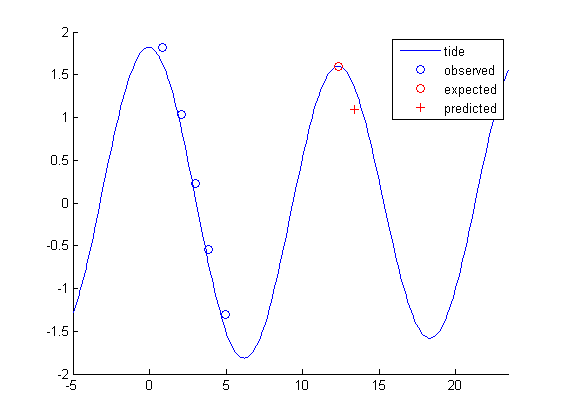
\includegraphics[width=0.6\textwidth]{edge_lin_1.png}
		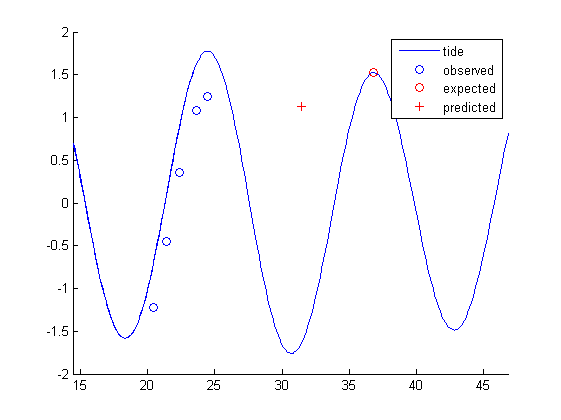
\includegraphics[width=0.6\textwidth]{edge_lin_2.png}
		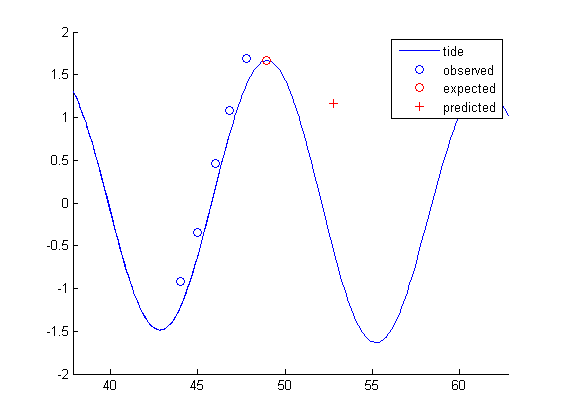
\includegraphics[width=0.6\textwidth]{edge_lin_3.png}
		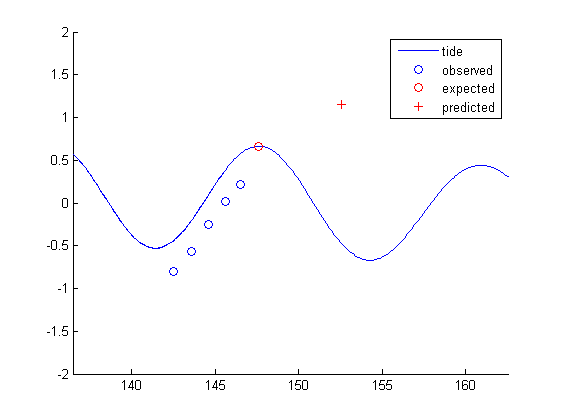
\includegraphics[width=0.6\textwidth]{edge_lin_4.png}
		\FloatBarrier
		
	\section{Predizione con Multilayer Perceptron}
		Il seguente tentativo è stato con una rete Feed-Forward, in particolare un Multilayer Perceptron.\\
		\\
		Si è subito notato come questo tipo di rete risponda molto meglio alla predizione del prossimo picco di marea rispetto alla rete lineare di Widrow, quindi si è cercato di trovare il \underline{minimo numero di neuroni} dello strato nascosto affinché l'errore medio totale potesse scendere sotto un valore accettabile, che ci è sembrato opportuno fissare al \textbf{12\%}.\\
		Il risultato è stato che \textbf{6 neuroni} rappresentano il minimo per avere un errore minore uguale a \textbf{1.02}, che corrisponde appunto al \textbf{12\%} su 8.5. Ovviamente, più neuroni fanno scendere ulteriormente l'errore, ma la crescita è molto lenta rispetto al numero di neuroni necessari, quindi il 12\% di errore con 6 neuroni sembra essere un buon compromesso.\\
		\\
		Per riprodurre tale simulazione si veda il Codice \ref{lst:tideFFEdge}.\\
		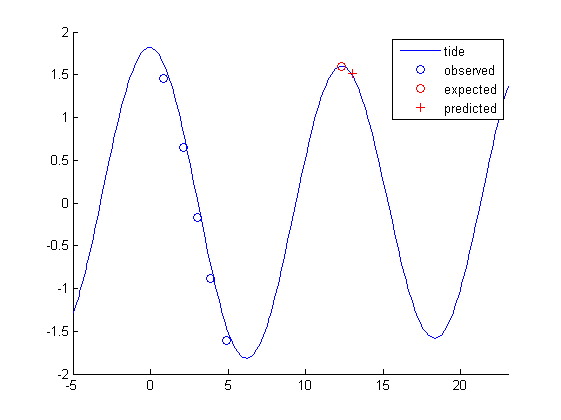
\includegraphics[width=0.6\textwidth]{edge_ff_1.png}
		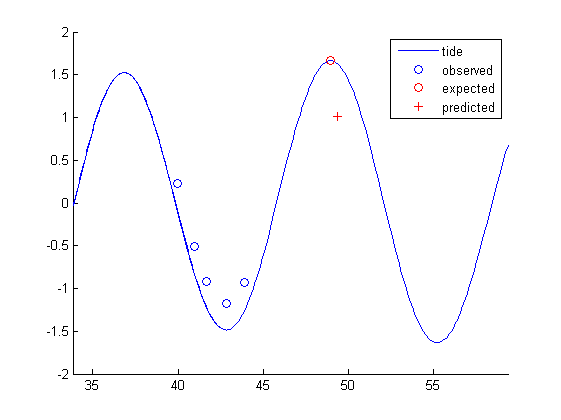
\includegraphics[width=0.6\textwidth]{edge_ff_2.png}
		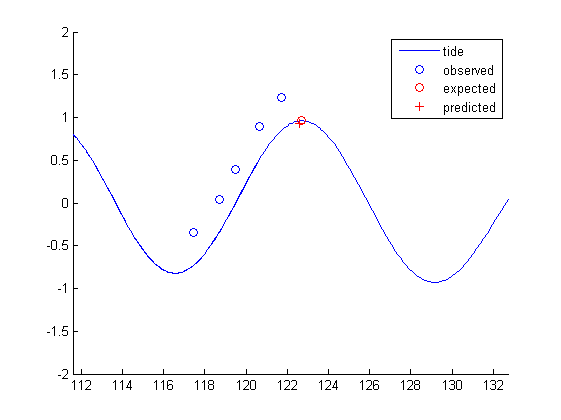
\includegraphics[width=0.6\textwidth]{edge_ff_3.png}
		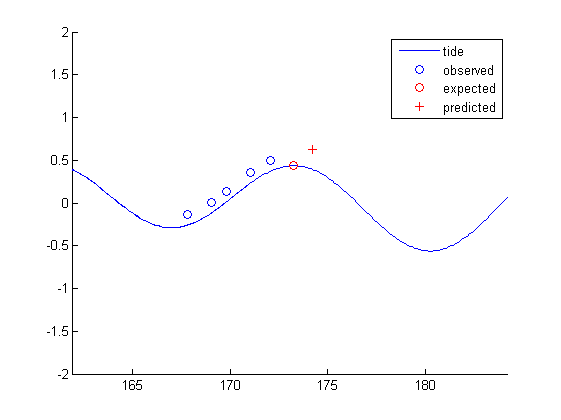
\includegraphics[width=0.6\textwidth]{edge_ff_4.png}
		\FloatBarrier